\documentclass[conference]{IEEEtran}
\usepackage{graphicx}
\usepackage[caption=false,font=footnotesize]{subfig}

\begin{document}

\begin{figure*}[t]
\centering

% -------- Row 1 --------
\subfloat[]{%
\raisebox{0pt}{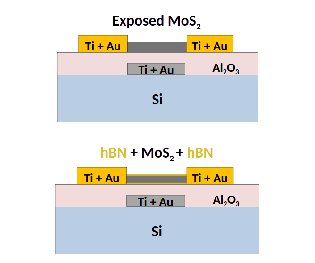
\includegraphics[]{figures/crossections.pdf}}
}
\hfill
\subfloat[]{%
\raisebox{0pt}{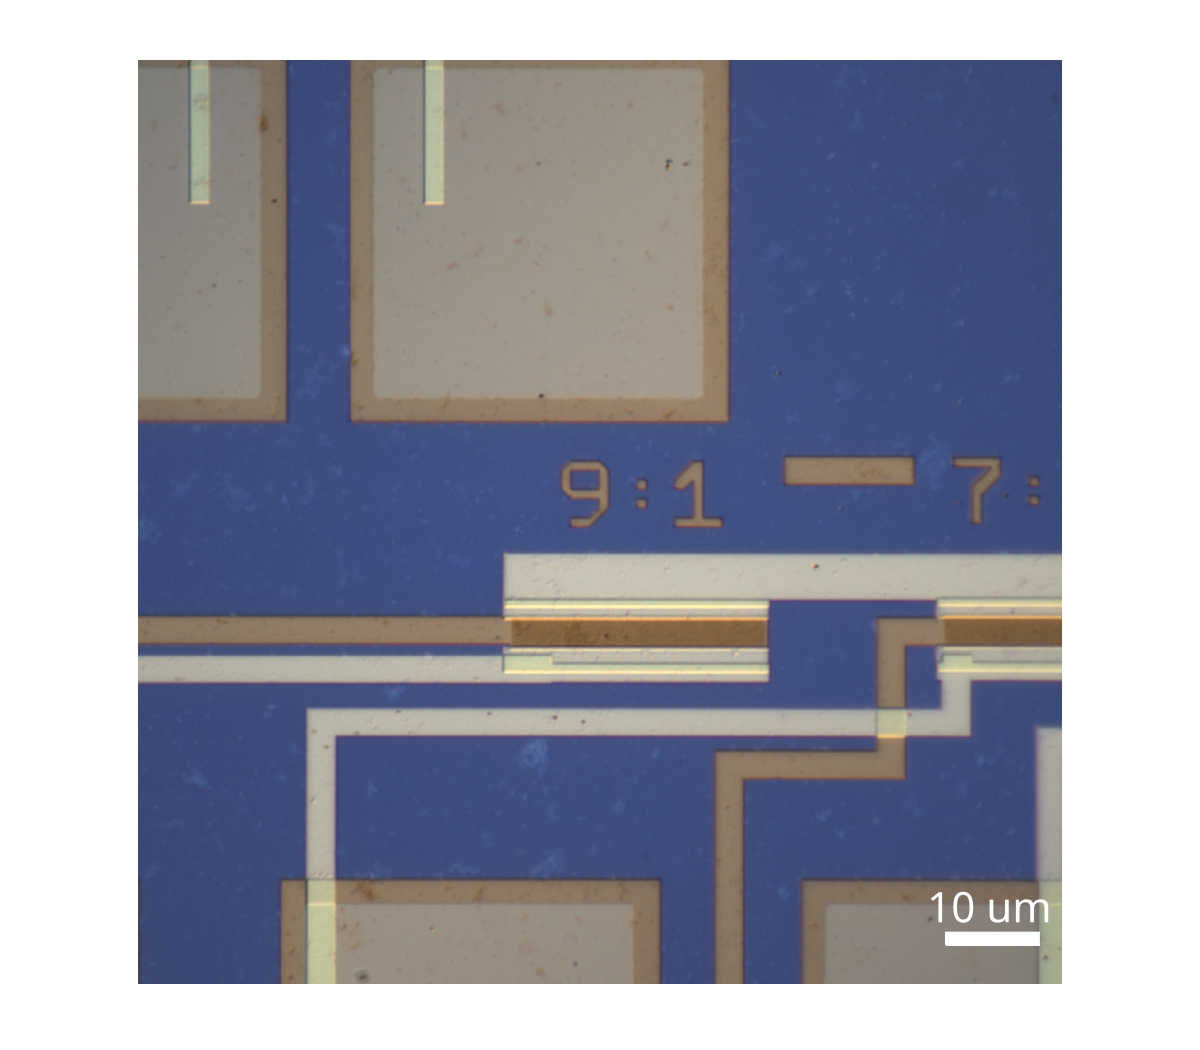
\includegraphics[]{figures/OM_FET.pdf}}
}
\hfill
\subfloat[]{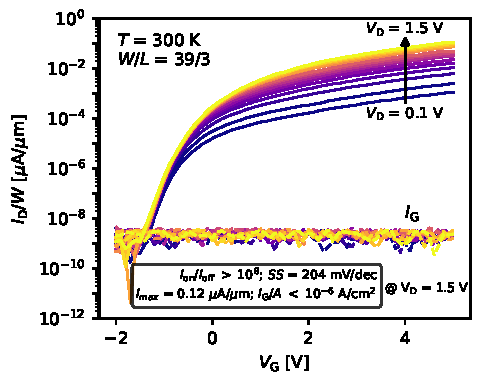
\includegraphics[]{figures/IdVg_encapsulated_1.pdf}}\\[-0.9em]

% -------- Row 2 --------
\subfloat[]{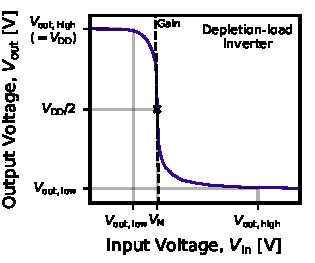
\includegraphics[]{figures/inverter_VTC.pdf}}

\hfill
\subfloat[]{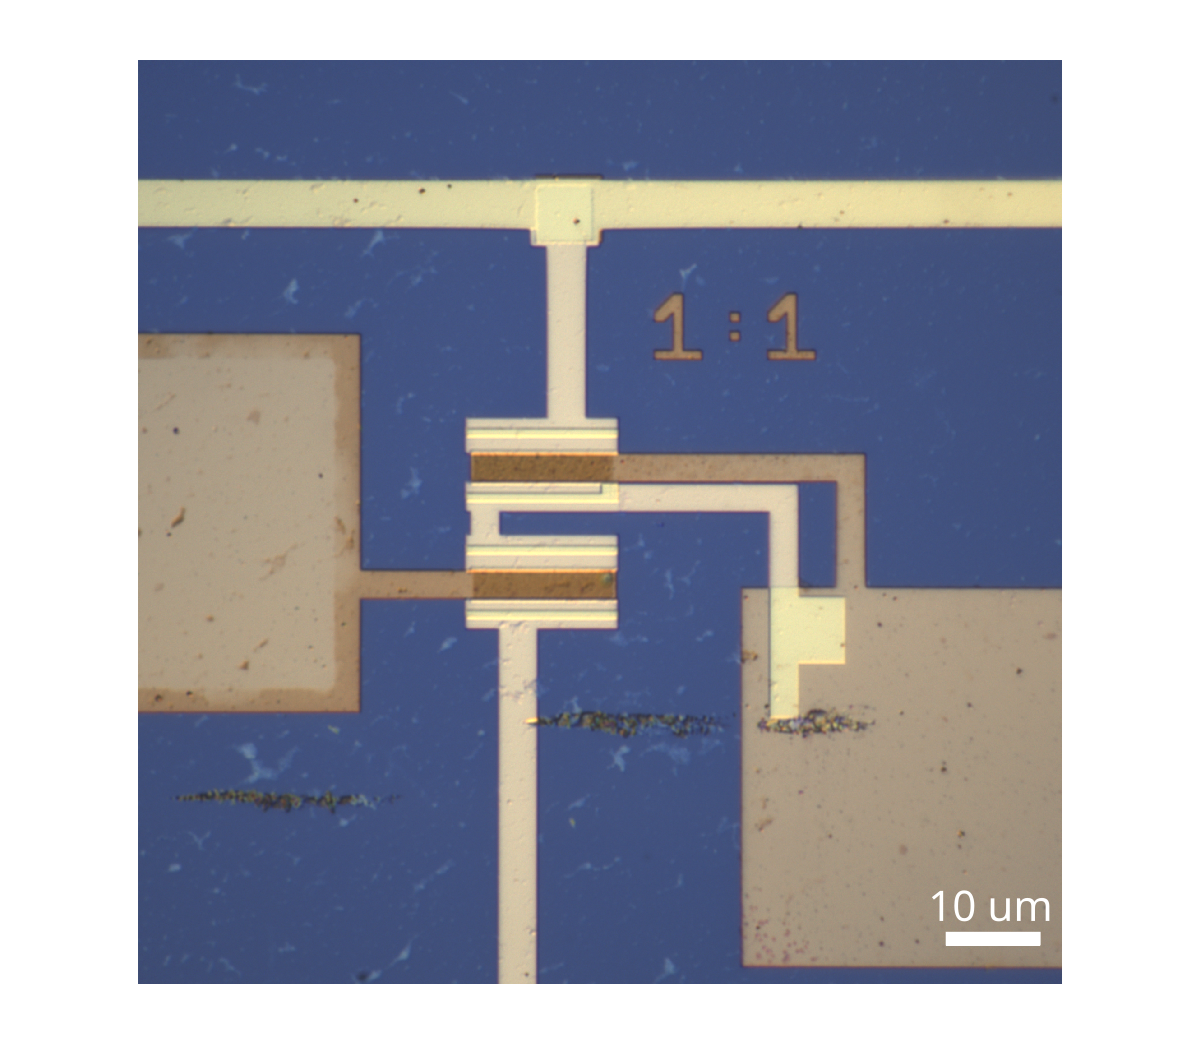
\includegraphics[]{figures/OM_INV.pdf}}

\hfill
\subfloat[]{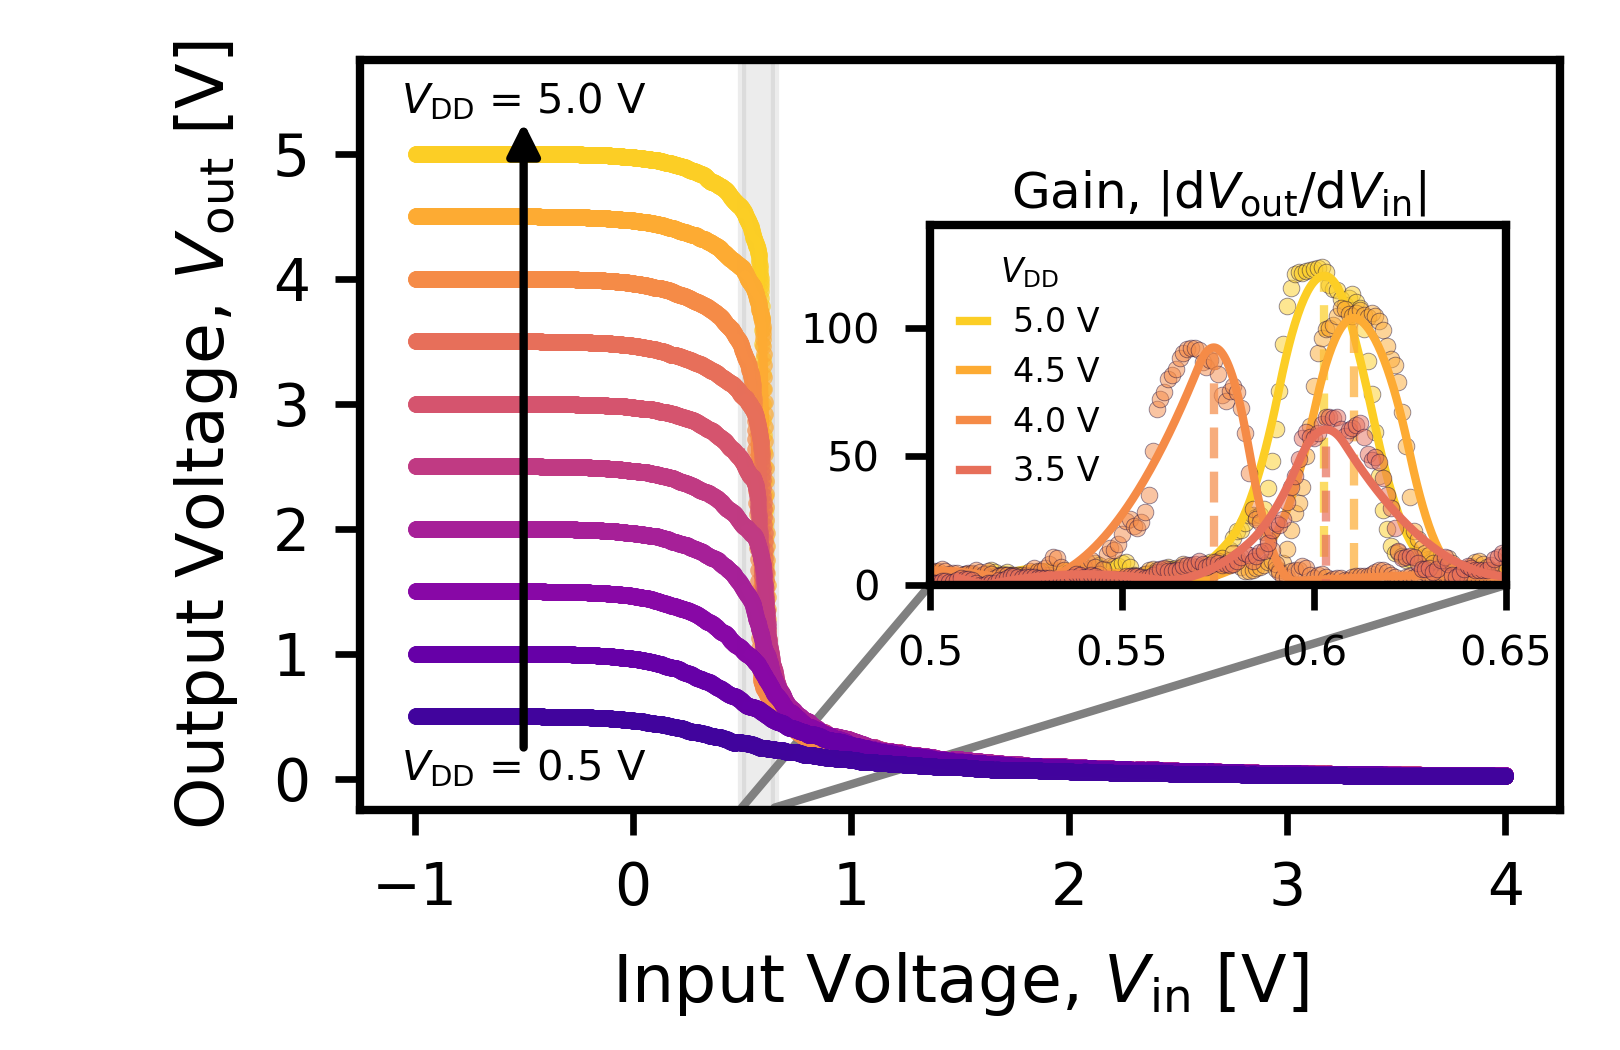
\includegraphics[]{figures/inverter_gain.png}
}

\vspace{-2pt}

\caption{%
(a)~\textbf{Device cross-section:} Schematics of exposed (top) and hBN-encapsulated (bottom) MoS$_2$ FETs.
(b)~\textbf{FET optical image:} Fabricated hBN-encapsulated FET.
(c)~\textbf{Performance of the fabricated devices:} $I_\mathrm{D(G)}$--$V_\mathrm{G}$ curves for different drain voltages and key device metrics extracted at $V_\mathrm{D}$ = 1.5 V.
(d)~\textbf{Inverter VTC:} Typical voltage transfer curve of a depletion-load nMOS inverter.
(e)~\textbf{Inverter optical image:} Fabricated hBN-encapsulated inverter.
(f)~\textbf{Inverter performance with $V_\mathsf{DD}$:} Inverter VTC curves for different supply voltages and the corresponding gain curves for the higher supply voltages.
}
\label{fig:devices_fabrication_performance}

\vspace{-8pt}
\end{figure*}
\end{document}